\section{Estado del arte}

En la intersección entre el avance tecnológico y el envejecimiento de la población, los juegos digitales emergen como una herramienta multifacética con el potencial de promover el bienestar y la calidad de vida de los adultos mayores. El estado del arte representa una síntesis dinámica de la investigación, desarrollo y aplicaciones existentes en este campo en constante evolución.

En esta revisión, se explorarán las principales tendencias y avances en cuatro áreas clave: los juegos serios, diseñados con objetivos específicos de aprendizaje o rehabilitación; los juegos digitales, adaptados para satisfacer las necesidades y preferencias de las personas mayores; el estado actual de las tecnologías aplicadas, incluyendo dispositivos y software especializado en el diseño y finalmente, ejemplos de aplicaciones prácticas desarrolladas en esta línea de investigación.

\subsection{Juegos serios}

Los juegos \textit{serios} se distinguen por su enfoque principal en objetivos educativos o formativos, relegando la diversión a un segundo plano \parencite{juegosSerios}.
Mientras que los juegos tradicionales buscan principalmente entretener al jugador, los juegos serios utilizan la pedagogía para integrar la instrucción dentro de la experiencia de juego. Esto implica que, aunque la diversión sigue siendo un elemento presente, el aprendizaje se convierte en el objetivo primordial.

\subsubsection{Origen de los juegos serios}

Hay que remontarse al año 1970 para datar la fecha de aparición del término juego serio o \textit{serious game}. En el contexto de los juegos de mesa, Clark Abt, investigador de EEUU publicó un libro titulado \enquote{\textit{Serious Games}} \parencite{juegosSerios5}, en el que explora las formas en que los juegos pueden utilizarse para instruir e informar. Utiliza enfoques innovadores para la resolución de problemas mediante técnicas de juego en contextos tan diferentes como el aprendizaje de las matemáticas, ciencias sociales y física o las tareas de planificación en el gobierno y la industria.

Pero no es hasta 2002 cuando el concepto de juego serio, tal como se conoce hoy en día, se recoge por Ben Sawyer
y David Rejeski en un artículo sobre los juegos serios en el ámbito de la política pública \parencite{juegosSerios6}, que tuvo un gran impacto, gracias a la creación de una asociación para promover el uso de los videojuegos con un propósito serio. Dicha asociación, Serious Games Initiative, de la cuál es cofundador Sawyer a través del Woodrow Wilson Center continúa activa en la actualidad \parencite{juegosSerios4}.

Precisamente, es Ben Sawyer quien establece como primer juego serio el videojuego America’s Army \parencite{juegosSerios7}, un simulador de combate para instruir a militares en el campo de batalla a través de la realización de diferentes misiones.


\subsubsection{Concepto de juego serio}
Los juegos serios son una categoría de videojuegos desarrollados principalmente para propósitos educativos y formativos, aunque también pueden tener elementos de entretenimiento. Estos juegos se distinguen por su enfoque en la transmisión de conocimientos y habilidades, a menudo relacionados con temas como la política, la salud, el entrenamiento militar, la educación, el ámbito empresarial, etc  \parencite{juegosSerios3}.

Se listan a continuación algunas de las características principales que distinguen a los juegos serios del resto:

\begin{itemize}[leftmargin=1.5cm, topsep=0pt, itemsep=1pt, after=\vspace{0pt}]
    \item \textbf{Fin educativo}: su principal objetivo es la formación en lugar del entretenimiento. La adquisición de habilidades técnicas y comprensión de procesos complejos.
    \item \textbf{Realismo}: están vinculados a aspectos de la realidad, favoreciendo la identificación del jugador con el contexto que se está simulando.
    \item \textbf{Ambiente virtual seguro}: proporcionan un entorno tridimensional virtual seguro para la práctica en ciertas áreas, como el entrenamiento militar.
    \item \textbf{Interés temático}: pueden abordar temas políticos, económicos, psicológicos, religiosos, entre otros, a menudo con un enfoque en la educación y el entrenamiento.
\end{itemize}

Los siguientes son algunos ejemplos reales y de ámbito específico de videojuegos serios:
\begin{itemize}[leftmargin=1.5cm, topsep=2.2pt, itemsep=1pt]
    \item \textbf{Biomedical Training}: entrenamiento para trabajadores de la salud en emergencias.
    \item \textbf{Food Force}: educación sobre el Programa Mundial de Alimentos de la ONU.
    \item \textbf{Incident Commander}: dirección de acciones en crisis sociales y desastres naturales.
    \item \textbf{Hazmat: Hotzone}: simulación para bomberos en situaciones de emergencia.
    \item \textbf{Yourselfittness}: regímenes de ejercicios físicos y aeróbicos.
    \item \textbf{Real Life 2007}: simulación global para entender condiciones de vida en diferentes países.
\end{itemize}

Los juegos serios son una herramienta poderosa para el aprendizaje y la formación en distintos campos. Involucran principios pedagógicos y cognitivos para garantizar un entrenamiento efectivo y ofrecen diversas ventajas como la familiarización con interfaces tecnológicas y la mejora de habilidades necesarias para la sociedad digital.

En el contexto de los adultos mayores, los videojuegos serios pueden resultar valiosos para el mantenimiento cognitivo, la estimulación mental y la mejora de habilidades específicas.

\newpage
\subsubsection{Juegos serios en la rehabilitación neuropsicológica}

Cabe destacar el papel de los juegos serios en el ámbito de la informática médica, en concreto, en el entrenamiento y la rehabilitación neuropsicológica.  \enquote{En la rehabilitación cognitiva los retos de un juego serio por lo general inciden directamente en un déficit específico, lo que puede repercutir al mismo tiempo en más de uno} \parencite{juegosSerios2}.

En los últimos años, ha habido un notable aumento en la investigación y desarrollo de juegos computarizados para la rehabilitación cognitiva. Ejemplos como RehaCom® y Gradior® \parencite{ICTestudios} han demostrado resultados positivos en varios centros de salud al ofrecer una variedad de ejercicios digitales que abordan áreas cognitivas clave como la atención, la percepción, la memoria y el lenguaje. 

\begin{figure}[ht]
    \centering
    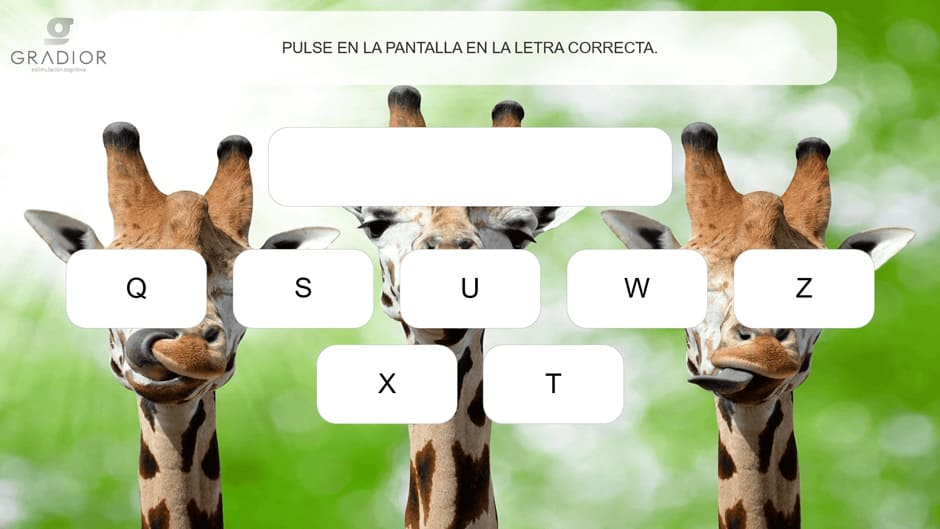
\includegraphics[width=0.8\textwidth]{imgs/gradior.jpg}
    \caption{Gradior, un sistema de evaluación y rehabilitación neuropsicológica}
    \label{fig:gradior}
\end{figure}

Otro destacado ejemplo es el módulo EINK de RehaCom®, diseñado para tratar déficits de memoria de trabajo y planificación mediante la simulación de situaciones diarias, como ir de compras. Estos programas permiten adaptar la intervención terapéutica a las necesidades de cada paciente, ajustando la dificultad y la retroalimentación sobre su progreso.

En resumen, los juegos serios ofrecen una vía innovadora y efectiva para abordar las deficiencias cognitivas, a la vez que mantienen la motivación del paciente durante las sesiones de tratamiento.

\newpage
\subsubsection{Juegos tradicionales en grupo y sus ventajas cognitivas}

A continuación, se nombrarán algunos juegos tradicionales y populares que fomentan el contacto social y evitan el deterioro cognitivo en personas mayores, especialmente trabajando la memoria. Dado que esto es justo lo que se busca lograr con este proyecto, estas actividades servirán como fuente de inspiración para la conceptualización y desarrollo del mismo \parencite{juegosMem2}.

\begin{itemize}[leftmargin=1.5cm, topsep=2.2pt, itemsep=0.5pt]
    \item \textbf{Cada oveja con su pareja}: 
    consiste en agrupar objetos en función de su categoría, utilizando todo tipo de elementos. Desde las cartas de una baraja para agrupar por palos, hasta objetos aleatorios dispuestos, como frutas, verduras... Contribuye a mantener la capacidad intelectual, la memoria y la coordinación visual y manual.
    \item \textbf{Veo-veo}:
    juego mítico que hace las delicias de los más pequeños, y suele ser cuando juegan con alguien más mayor. Uno de los jugadores tendrá que adivinar el objeto elegido por su inicial; se pueden dar pistas sobre el lugar de la sala en que se encuentra.
    \item \textbf{Palabras encadenadas}:
    se trata de coger la última sílaba de una palabra y encadenar con la siguiente; que la última sílaba de esa palabra sea la primera de la siguiente. Fomenta la memoria y la comunicación, además de la atención y la concentración.
    \item \textbf{Puzzle de refranes}: 
    los adultos mayores son grandes conocedores de refranes populares. El juego consistirá en escribir los refranes en dos partes, en trozos de papel separados. Los jugadores deberán enlazar cada parte para completar el refrán, que puede ir orientado a una temática y luego formar un mural.
    \item \textbf{Quién es quién}:
    cada persona es asignada una palabra que todos menos él conocen. Dicha persona tendrá que ir haciendo preguntas de sí o no hasta adivinar quién o qué es.
    \item \textbf{Adivina la canción}:
    se pueden tomar como referencia las canciones más escuchadas del tiempo en el que las personas mayores eran jóvenes. Se reproducirá la canción durante un corto espacio de tiempo y los participantes anotarán el nombre y artista de la canción. Agudeza auditiva, rapidez y capacidad de atención son algunos de sus beneficios.
\end{itemize}

También destacan juegos de mesa como el Scrabble (creatividad y habilidades lingüísticas), Dominó (planificación y estrategia), Bingo (atención y memoria a corto plazo), Pictionary (comunicación no verbal), rompecabezas (concentración y paciencia), etc \parencite{juegos-mesa}.

\subsection{Juegos digitales para adultos mayores}

Una vez explicado el concepto de juego serio y algunos ejemplos concretos, se hará hincapié en un tipo concreto del mismo: los juegos digitales, que deben su nombre a la tecnologías de digitalización en las que están basados.

Los juegos digitales representan una herramienta innovadora y prometedora para abordar los desafíos asociados con el envejecimiento activo y saludable expuestos anteriormente. A través de dispositivos como computadoras, tabletas, consolas de juegos y teléfonos inteligentes, los adultos mayores tienen acceso a una amplia variedad de experiencias de juego que pueden contribuir a su bienestar físico, cognitivo y social.

Muchos de los juegos digitales populares entre adultos mayores están basados en juegos tradicionales, pues la familiaridad de las dinámicas es un factor que contribuye a su popularidad. Ejemplos de aplicaciones:
\begin{itemize}[leftmargin=1.5cm, topsep=2.2pt, itemsep=0.4pt]
    \item \textbf{Sudoku}: el clásico juego de números ayuda a ejercitar la mente y la concentración.
    \item \textbf{Wordscapes}: búsqueda de palabras que desafía la agilidad mental y el vocabulario.
    \item \textbf{Candy Crush Saga}: niveles de rompecabezas que pueden ser adictivos y desafiantes.
    \item \textbf{Jigsaw Puzzles}: selecciones de rompecabezas virtuales de diferentes niveles de dificultad.
    \item \textbf{Solitaire}: versión digital del clásico juego de cartas, fácil de aprender y entretenido.
    \item \textbf{Peak – Brain Games and Training}: variedad de juegos diseñados para ejercitar diferentes áreas del cerebro.
    \item \textbf{Neurona App}: aplicación que pretende estimular atención, memoria, razonamiento y planificación de adultos mayores mediante diversos juegos.
    \item \textbf{Fit Brain Trainer}: cuenta con 360 juegos de agilidad mental, memoria, capacidad visual y de deducción.
    \item \textbf{NeuroNation}: capaz de personalizar el entrenamiento para cada usuario \parencite{juegosMem1}.
\end{itemize}

Estos juegos son populares entre adultos mayores debido a su accesibilidad, puesto que son apps que pueden ser descargadas fácilmente en dispositivos móviles y tablets; tienen capacidad para ejercitar la mente, ya que la mayoría estimulan partes del cerebro concretas (la memoria, atención y resolución de problemas) y ofrecen entretenimiento sin demasiada complejidad al tener mecánicas de juego bastante simples.

La investigación en este campo se centra en comprender cómo los juegos digitales pueden promover el envejecimiento activo al mantener la mente activa, mejorar la destreza manual y fomentar la interacción social. Además, se busca diseñar juegos que sean accesibles y atractivos para esta población, teniendo en cuenta las necesidades y preferencias específicas de los adultos mayores.

A medida que la tecnología avanza y la aceptación de los juegos digitales entre los adultos mayores aumenta, resulta importante explorar cómo estos juegos pueden desarrollarse e integrarse de manera efectiva para mejorar la calidad de vida de esta población.


\subsubsection{El proyecto WorthPlay}

En este campo de investigación, destaca, entre otros, el proyecto \textit{WorthPlay} \parencite{WorthPlay2012}, que se enfoca en la investigación y desarrollo de juegos digitales para personas mayores, con el propósito de promover un envejecimiento activo y saludable. En él se reconoce que las tecnologías de la información y la comunicación (TIC) tienen el potencial de reducir el aislamiento social y mejorar el bienestar físico y psicosocial de los adultos mayores.

Para asegurar la efectividad de los juegos digitales, se destaca la necesidad de entender qué aspectos hacen que un juego valga la pena para esta población. Esto implica considerar elementos educativos, de socialización y de entretenimiento, así como la diversidad de preferencias en cuanto a la jugabilidad y el formato del juego.

\enquote{El proyecto se basa en el campo de la Interacción Persona-Ordenador (IPO), que busca mejorar la experiencia del usuario con las TIC. Se identifican tres olas en la investigación de IPO, desde la ergonomía hasta la experiencia de usuario (UX). WorthPlay se sitúa en la tercera ola, centrándose en la experiencia de juego y la participación del usuario durante un período prolongado en entornos reales} \parencite{WorthPlay2012}.

La investigación también se enfoca en la inclusión social y la superación de barreras de accesibilidad, como la destreza cognitiva y motriz. Se reconocen los estereotipos negativos sobre los adultos mayores en el contexto de los juegos digitales, y se busca desafiar estos estereotipos a través del diseño participativo de juegos.

El proyecto WorthPlay sigue un enfoque parecido al de este proyecto, ya que se basa en investigar y desarrollar prototipos de juegos destinados al envejecimiento activo y saludable de las personas mayores. Concretamente, hace hincapié en los juegos cognitivos, que estimulan el pensamiento y aprendizaje, y los de socialización, promoviendo las interacciones dentro del juego. Estos dos son justamente los puntos clave en los que debe centrarse el juego a implementar.

Se espera que este enfoque, seguido tanto en el proyecto Worthplay como en el desarrollo de este TFG, genere resultados significativos, contribuyendo a una mejor comprensión de las necesidades y preferencias de los adultos mayores en este campo.

\subsubsection{El juego digital \textit{Solitaire Quizz}}

jj

\subsection{Estado del arte de los asistentes virtuales}

En esta sección, se hablará sobre el estado actual de los asistentes virtuales, que se caracteriza por su creciente sofisticación impulsada por la IA, su diversidad en términos de funciones y aplicaciones, y la presencia destacada de plataformas líderes como Alexa, que continúan innovando y expandiendo las fronteras de esta tecnología.

\subsubsection{Influencia de la IA y clasificación}

La inteligencia artificial (IA) es una tecnología que ha evolucionado rápidamente y se ha integrado en la vida cotidiana de las personas, especialmente en la automatización de servicios y la toma de decisiones. Ha encontrado aplicaciones en diversos sectores, como la educación, la salud, la economía y la política, transformando la forma en que se prestan servicios y se interactúa con las organizaciones.

El aumento de la población y el crecimiento exponencial de las ciudades requieren sistemas más rápidos y eficientes para la atención al cliente. A raíz de esta necesidad, se han desarrollado asistentes virtuales inteligentes.

Un asistente virtual es un software con acceso a recursos en línea que emplea técnicas de IA y procesamiento del lenguaje natural para proporcionar soporte en tiempo real a usuarios y otorgar acceso a información relevante sobre los servicios ofrecidos por organizaciones públicas y privadas \parencite{tfgAlexa1}.

La arquitectura de estos sistemas se ha perfeccionado con el tiempo, desde ELIZA, precursor que emulaba a un psicoterapeuta, hasta los chatbots avanzados y versátiles de hoy en día, compatibles con múltiples dispositivos (altavoces, televisores, teléfonos móviles, tablets, etc).

En cuanto a la clasificación, existe más de un criterio para definir de los tipos de asistentes virtuales, pero los principales son los mencionados en el Cuadro \ref{tab:criterios_asistentes_virtuales}: según el grado de interacción con los usuarios, las funciones y finalidades del servicio, los medios de interacción y el grado de afectividad \parencite{asistentesConv}.

\begin{table}[H]
    \centering
    \begin{tabular}{|l|l|}
    \hline
    \rowcolor{lightgray}
    \textbf{Criterio} & \textbf{Tipos} \\
    \hline
    \multirow{2}{*}{Grado de interacción} & - Dirigidos \\
     & - Conversacionales \\
    \hline
    \multirow{3}{*}{Funciones y finalidades} & - Comunicación y marketing \\
     & - Atención al cliente \\
     & - Mejora de procesos \\
    \hline
    \multirow{3}{*}{Medios de interacción} & - Texto \\
     & - Multimedia \\
     & - Voz \\
    \hline
    \multirow{2}{*}{Grado de afectividad} & - No emocionales \\
     & - Emocionales \\
    \hline
    \end{tabular}
    \caption{Clasificación de asistentes virtuales}
    \label{tab:criterios_asistentes_virtuales}
\end{table}

\begin{itemize}[leftmargin=1.5cm, topsep=2pt, itemsep=1pt]
    \item \textbf{Dirigidos}: realizan preguntas predefinidas a los usuarios mediante elementos fijos, controlando la interacción con el usuario.
    \item \textbf{Conversacionales}: permiten una mayor libertad en las preguntas que el usuario quiere hacer, promoviendo una interacción más natural.
    \item \textbf{Comunicación y marketing}: brindan servicios de consulta dentro de aplicaciones móviles o web.
    \item \textbf{Atención al cliente}: asisten a los usuarios resolviendo sus dudas y consultas a través de conversaciones continuas.
    \item \textbf{Mejora de procesos}: tienen el objetivo de reducir el tiempo dedicado a una área específica.
    \item \textbf{No emocionales}: son los chatbots tradicionales y se limitan a dar respuestas oportunas a las solicitudes del usuario.
    \item \textbf{Emocionales}: diseñados para interactuar y comprender a las personas a través de conversaciones informales, permitiendo una atención personalizada.
\end{itemize}

Con respecto a las tendencias en el desarrollo e implementación de asistentes virtuales en organizaciones públicas y privadas, se observa que actualmente se utilizan asistentes dirigidos, el tipo más dominante es el de atención al cliente, el medio de interacción más empleado es el texto y suelen ser son no emocionales.

\subsubsection{Alexa, el asistente conversacional más extendido hoy en día}

Junto con Siri (Apple) y Google Assistant, Alexa, desarrollada por Amazon, es sin lugar a dudas una de los asistentes virtuales por voz más extendidas. Numerosos estudios confirman el creciente índice de uso e impacto en el mercado que ha supuesto el lanzamiento de Alexa, entre ellos los resultados obtenidos en la clasificación por puntuaciones del \textit{Voice Platform Impact Rating} (\autoref{fig:grafico-asistentes}).

\begin{figure}[H]
    \centering
    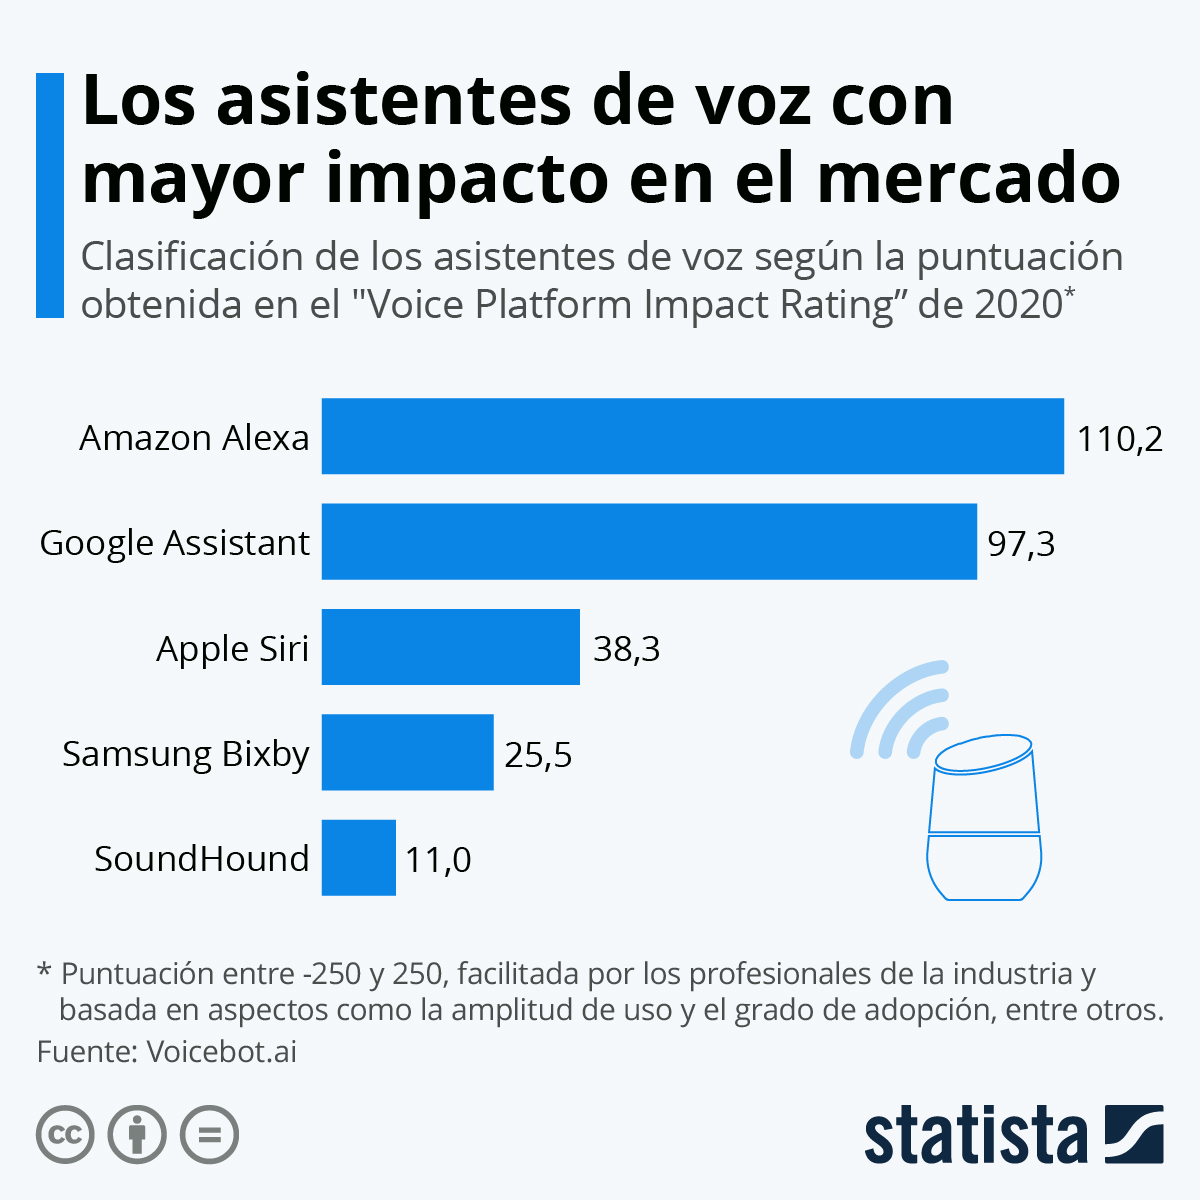
\includegraphics[width=0.5\textwidth]{imgs/grafico-asistentes.jpeg}
    \caption{Ranking de asistentes de voz según el VPIR en 2020 (\href{https://es.statista.com/grafico/22578/clasificacion-de-los-asistentes-de-voz/}{statista})}
    \label{fig:grafico-asistentes}
\end{figure}

Alexa fue lanzado en noviembre de 2014, se encuentra alojado en la nube de Amazon y está disponible en una gran variedad de dispositivos, incluyendo Amazon Echo y Echo Plus, así como también en dispositivos de terceros como smartphones, Raspberry Pi y vehículos.

Actualmente, cuenta con una amplia gama de funciones predefinidas, como manejo de alarmas, notificaciones, calendarios y búsqueda en internet para responder preguntas. Sin embargo, su verdadero potencial radica en las \textit{skills}, similares a aplicaciones de terceros que amplían sus funcionalidades, permitiendo interactuar con distintas compañías y acceder a sus servicios desde un mismo lugar. A nivel mundial, Alexa cuenta con más de 56,000 skills disponibles \parencite{tfgAlexa2}.

Las \textit{skills} de Alexa para el desarrollo de juegos ofrecen una amplia gama de posibilidades para crear experiencias interactivas y entretenidas. Estas habilidades permiten a los desarrolladores crear juegos de diferentes géneros y niveles de complejidad, desde simples juegos de palabras y adivinanzas hasta juegos de aventuras o trivial más elaborados.

Por los motivos mencionados anteriormente, se va a elegir a Alexa como la asistente virtual para el juego a desarrollar.

\subsection{Aplicaciones similares con asistentes de voz}

Se han visto algunas aplicaciones dirigidas a adultos mayores para favorecer su envejecimiento saludable en secciones anteriores, y ahora se mencionarán ejemplos de aplicaciones similares con asistentes conversacionales. 

\subsubsection{CELIA, mucho más que una asistente}

Existen algunas iniciativas dirigidas a las personas mayores que están en situación de aislamiento como el asistente virtual Celia (\href{https://celiatecuida.com/}{web oficial Celia}), desarrollado por personal del Centro de Investigación en Tecnologías de Telecomunicación de la Universidade de Vigo, atlanTTic, que ya se ha puesto en marcha con éxito ya que su uso es muy sencillo \parencite{celia-app}.

Las personas interesadas pueden acceder a este asistente virtual desde su teléfono móvil a través de la aplicación gratuita de CELIA (\autoref{fig:celia}), y también por WhatsApp, enviando un mensaje de texto o una nota de voz de manera que establecen una conversación con <<Celia>>. De esta sencilla manera  la persona  mayor que vive sola puede preguntar al asistente virtual al levantarse <<¿Qué tiempo va a hacer hoy?>> y buscar actividades para acudir como exposiciones, conferencias, conciertos que sean al aire libre o en espacios cubiertos dependiendo de la climatología. 

\begin{figure}[H]
    \centering
    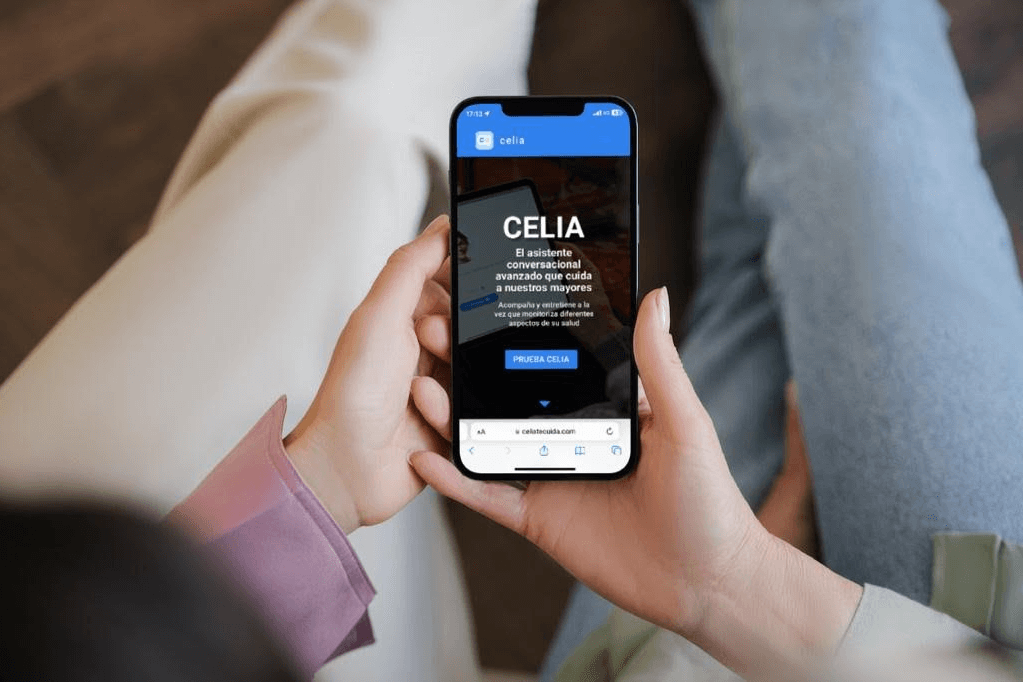
\includegraphics[width=0.55\textwidth]{imgs/celia.jpg}
    \caption{Celia, una asistente todoterreno 24 horas al día.}
    \label{fig:celia}
\end{figure}

Esta aplicación es útil para la ejecución de comandos básicos y ayuda a las personas mayores, pero no ofrece la capacidad de personalización de un juego digital centrado en promover el envejecimiento activo de los adultos mayores, además de no estar pensado para el uso de más de una persona a la vez.

\subsubsection{Juego de los trayectos orientado a la detección del deterioro cognitivo}

Es una aplicación (o skill) basada en Alexa que puede usarse como una herramienta clínica destinada a la evaluación de la capacidad de memoria de trabajo en pacientes. El juego implementado consiste en ir memorizando las calles de Jaén de una ruta seleccionada aleatoriamente del mapa cada vez que se inicia una partida \parencite{tfgAlexa3}.

Es compatible y accesible a través de cualquier dispositivo de la familia de Alexa y viene con un sistema robusto de almacenamiento en la nube, diseñado para almacenar de manera segura y eficiente toda la información de los usuarios y sus interacciones con el sistema.

El juego en sí consiste en que la persona usuaria, un adulto mayor, debe recordar secuencias en forma de nombres de calle, contestando a las preguntas formuladas por Alexa, quien es la encargada de pedirle nombres de calles o rutas para ejercitar su memoria. Se incluye un ejemplo de ejecución el la \autoref{fig:tfg-caminos-1}.

\begin{figure}[H]
	\centering
	
\includegraphics[width=0.6\textwidth]{imgs/tfg-caminos-1.JPG}
	\caption{Ejemplo de interacción con el juego de las rutas}
	\label{fig:tfg-caminos-1}
\end{figure}

Además, en los dispostivos de Alexa que tengan pantalla, se mostrará un soporte visual que incluye imágenes de las calles para ayudar a los jugadores y jugadoras, haciendo el juego más atractivo (\autoref{fig:tfg-caminos-2}).

\begin{figure}[H]
	\centering
	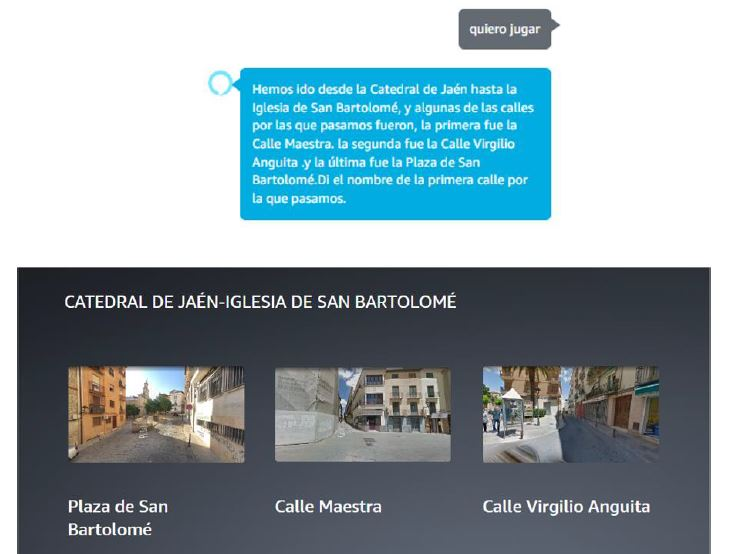
\includegraphics[width=0.8\textwidth]{imgs/tfg-caminos-2.JPG}
	\caption{Interacción con el juego de las rutas y su interfaz}
	\label{fig:tfg-caminos-2}
\end{figure}

Los resultados de las partidas y la información de los usuarios se almacenan en una base de datos y pueden ser consultados mediante una app complementaria, destinada exclusivamente al uso del especialista. Así, este último podrá evaluar de manera efectiva la capacidad de memoria de trabajo de sus pacientes, facilitando la detección rápida del deterioro cognitivo.

En cuanto a la estimulación cognitiva y accesibilidad, es una aplicación sólida y une buena fuente de inspiración para este proyecto; sin embargo, se echa en falta el aspecto social del juego, ya que está pensado para un solo jugador o jugadora. La aplicación a desarrollar en este proyecto sí tendrá en cuenta este factor, considerando no solo beneficios cognitivos, sino también vinculados a las relaciones sociales.

\subsubsection{Juegos serios y experiencias inclusivas}

El proyecto \enquote{Juegos serios y experiencias inclusivas} \parencite{tfgAlexa4} tiene como objetivo desarrollar dos juegos serios que promuevan el envejecimiento activo y el ejercicio cognitivo para personas mayores, utilizando el asistente de voz Alexa. Estos juegos están diseñados para ser accesibles y permitiendo que los participantes ejerciten sus habilidades cognitivas a la vez que se entretienen. A continuación, se describen los dos juegos desarrollados:

El primero, series de palabras, consiste en que el usuario debe recordar y repetir una serie de palabras que Alexa le dicta. Cada vez que repite correctamente la secuencia, se le añade una nueva palabra. Estas listas incluyen temas como colores, animales, países o una mezcla de los anteriores. Se muestra un ejemplo de partida en la \autoref{fig:tfg-juegos-1} y \ref{fig:tfg-juegos-11}: 

\begin{figure}[H]
	\centering
	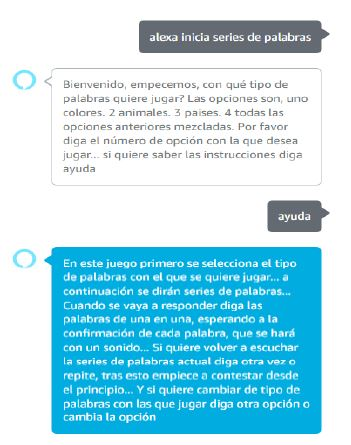
\includegraphics[width=0.6\textwidth]{imgs/tfg-juegos-1.JPG}
	\caption{Interacción con el juego de las series de palabras (1)}
	\label{fig:tfg-juegos-1}
\end{figure}

\begin{figure}[H]
	\centering
	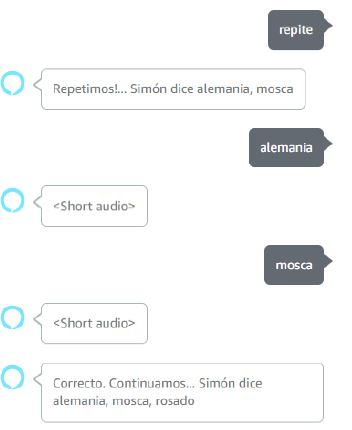
\includegraphics[width=0.6\textwidth]{imgs/tfg-juegos-11.JPG}
	\caption{Interacción con el juego de las series de palabras (2)}
	\label{fig:tfg-juegos-11}
\end{figure}

En el segundo juego (\autoref{fig:tfg-juegos-2}), Alexa plantea afirmaciones sobre diversos temas de cultura general, y el jugador debe responder si la afirmación es verdadera o falsa. Si el jugador tiene dudas, puede pedir una pista o saltarse la pregunta. Tras la respuesta, Alexa proporciona una breve explicación sobre la afirmación, tanto si fue correcta como incorrecta.

\begin{figure}[H]
	\centering
	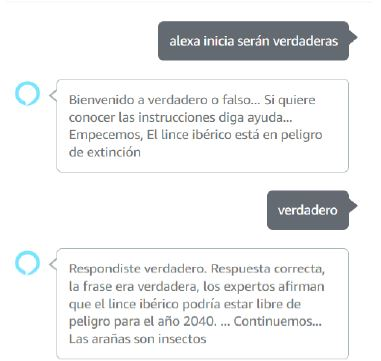
\includegraphics[width=0.6\textwidth]{imgs/tfg-juegos-2.JPG}
	\caption{Interacción con el juego de verdadero o falso}
	\label{fig:tfg-juegos-2}
\end{figure}

Como sucedía con la aplicación anterior, si bien es cierto que estos juegos ayudan a estimular la memoria tanto a corto plazo como largo, así como la concentración y razonamiento, no consideran la modalidad multijugador que podría beneficiar a su envejecimiento saludable.
